% !TEX root = calculus.tex

\chapter{CONVERGENT SEQUENCE}
\label{conv-seq}
{\parindent=0pt
\athr Let us prove the following theorem: 
\begin{mytheo}{Theorem}
If a sequence has a limit, it is bounded.
\label{limit-bound}
\end{mytheo}
We assume that $a$ is the limit of a sequence ($y_{n}$). Now take an arbitrary value of $\varepsilon$ greater than 0. According to the definition of the limit, the selected $\varepsilon$ can always be related to $N$ such that for all $n > N, \, Iy_{n} -a | < \varepsilon$ starting with $n = N + 1$, all the subsequent terms of the sequence satisfy the following inequalities
\begin{equation*}
a - \varepsilon < y_{n} < a + \varepsilon 
\end{equation*}
As to the terms with serial numbers from 1 to $N$, it is alway possible to select both the greatest (denoted by $B_{1}$ ) and the least (denoted by $A_{1}$) terms since the number of these term is \emph{finite}.

Now we have to select the least value from $a - \varepsilon$ and $A_{1}$ (denoted by $A$) and the greatest value from $a + \varepsilon$ and $B_{1}$ (denoted by $B$). It is obvious that $A \leqslant y_{n} \leqslant B$ for all the terms of our sequence, which proves that the sequence $y_{n}$ is bounded.

\rdr I see.

\athr Not too well, it seems. Let us have a look at the logical structure of the proof. We must verify that if the sequence has a limit, there exist two numbers $A$ and $B$ such that $A \leqslant y_{n} \leqslant B$ for each term of the sequence. Should the sequence contain a \emph{finite} number of terms, the existence of such two numbers would be evident. However, the sequence contains an \emph{infinite} number of terms, the fact that complicates the situation. 

\rdr Now it is clear! The point is that if a sequence has a limit $a$, one concludes that in the interval from $a - \varepsilon$ to $a + \varepsilon$ we have an infinite set of $y_{n}$ starting from $n = N +1$ so that \emph{outside of this interval} we shall find only a finite number of terms (not larger than $N$).

\athr Quite correct. As you see, the limit ``takes care of'' all the complications associated with the behaviour of the infinite ``tail'' of a sequence. Indeed, $| y_{n} - a | < \varepsilon$ for \emph{all} $n > N$, and this is the main ``delicate'' point of this theorem. As to the first $N$ terms of a sequence, it is essential that their set is finite.

\rdr Now it is all quite lucid. But what about $\varepsilon$ Its value is not preset, we have to select it.

\athr A selection of a value for $\varepsilon$ affects only $N$. If you	take a smaller $\varepsilon$,	you will get, generally speaking, a larger $N$. However, the number of the terms of a sequence which do not satisfy	$| y_{n} - a | < \varepsilon$ will remain finite.

And now try to answer the question about the validity of t.he converse theorem: If a sequence is bounded, does it imply it is convergent as well?

\rdr The converse theorem is not true. For example, sequence \eqref{series-10} which was discussed in the first dialogue is bounded. However, it has no limit.

\athr Right you are. We thus come to a corollary:
\begin{mytheo}{Corollary}
The boundedness of a sequence is a necessary condition for its convergence; however, it is not a sufficient condition. If a sequence is convergent, it is bounded. If a sequence is unbounded, it is definitely non-convergent,
\end{mytheo}

\rdr I wonder whether there is a sufficient condition for the convergence of a sequence?

\athr We have already mentioned this condition in the previous dialogue, namely, simultaneous validity of both the boundedness and monotonicity of a sequence. The \textbf{Weierstrass Theorem} states:
\begin{mytheo}{Weierstrass Theorem}
If a sequence is both bounded and monotonic, it has a limit.
\end{mytheo}
Unfortunately, the proof of the theorem is beyond the scope of this book; we shall not give it. I shall simply ask you to look again at sequences \eqref{series-05}, \eqref{series-07}, and \eqref{series-13} (see \hyperref[infinite-seq]{Dialogue One}), which satisfy the conditions of the Weierstrass theorem. 

\rdr As far as I understand, again the converse theorem is not true. Indeed, sequence \eqref{series-09} (from \hyperref[infinite-seq]{Dialogue One}) has a
limit but is not monotonic. 

\athr That is correct. We thus come to the following conclusion.
\begin{mytheo}{Conclusion}
If a sequence is both monotonic and bounded, it is a sufficient (but not necessary)	condition for its convergence.
\end{mytheo}

\rdr Well, one can easily get confused.

\begin{figure}[!h]
\centering
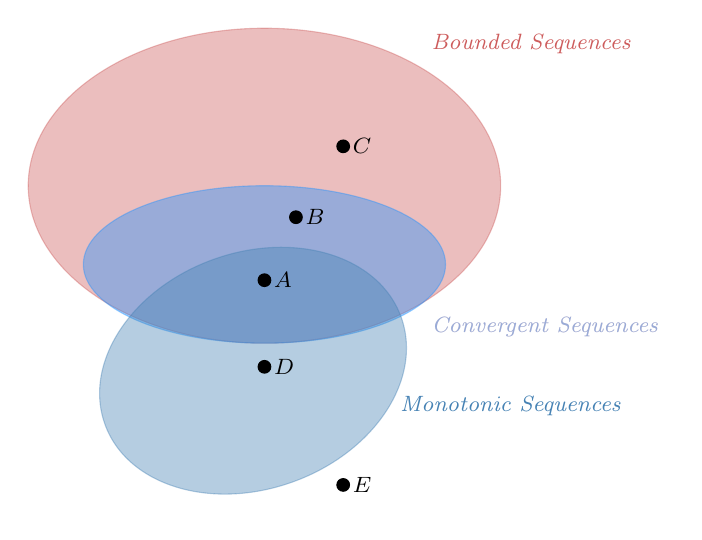
\begin{tikzpicture}[opacity=0.4]
  \filldraw [color=IndianRed=1.5,x radius=3cm, y radius=2cm](1,0) circle;
  \filldraw [color=DodgerBlue,radius=1.5,x radius=2.3cm, y radius=1cm](1,-1) circle;
  \filldraw [color=SteelBlue,radius=1.5,x radius=2cm, y radius=1.5cm,rotate=20](0,-2.5) circle;
\clip(0,-4) rectangle (6.2,2);
\draw (3,1.8) node[right,color=IndianRed,opaque] {\footnotesize \textit{Bounded Sequences}};
\draw (2.6,-2.8) node[right,color=SteelBlue,opaque] {\footnotesize \textit{Monotonic Sequences}};
\draw (3,-1.8) node[right,color=IndianRed] {\footnotesize \textit{Convergent Sequences}};
\draw (3,-1.8) node[right,color=DodgerBlue] {\footnotesize \textit{Convergent Sequences}};
\draw (1,-1.2) node[right,color=Black,opaque] {\footnotesize $A$};
  \filldraw [color=black,radius=0.8mm,opaque] (1,-1.2) circle;
\draw (1.4,-.4) node[right,color=Black,opaque] {\footnotesize $B$};
  \filldraw [color=black,radius=0.8mm,opaque](1.4,-.4) circle;
\draw (2,.5) node[right,color=Black,opaque] {\footnotesize $C$};
  \filldraw [color=black,radius=0.8mm,opaque](2,.5) circle;
\draw (1,-2.3) node[right,color=Black,opaque] {\footnotesize $D$};
  \filldraw [color=black,radius=0.8mm,opaque](1,-2.3)  circle;
\draw (2,-3.8) node[right,color=Black,opaque] {\footnotesize $E$};
  \filldraw [color=black,radius=0.8mm,opaque](2,-3.8) circle;
\end{tikzpicture}
%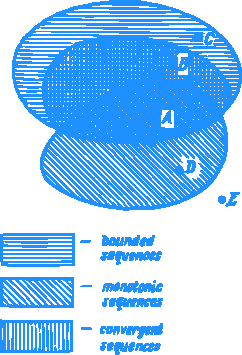
\includegraphics[width=0.4\textwidth]{figures/fig-08.pdf}
\caption{Bounded, monotonic and convergent sequences.}
\label{fig-08}
\end{figure}


\athr In order to avoid confusion, let us have a look at another illustration (\hyperref[fig-08]{Figure \ref{fig-08}}). Let us assume that all bounded sequences are ``collected'' (as if we were picking marbles scattered on the floor) in an area shaded by horizontal lines, all monotonic sequences are collected in an area shaded
by tilted lines, and, finally, all convergent sequences are collected in an area shaded by vertical lines. \hyperref[fig-08]{Figure \ref{fig-08}} shows how all these areas overlap, in accordance with the theorems discussed above (the actual shape of all the areas is, of course, absolutely arbitrary). As follows from the figure, the area shaded vertically is completely included into the area shaded horizontally. It means that \emph{any convergent sequence must be also bounded}. The overlapping of the areas shaded horizontally and by tilted lines occurs inside the area shaded vertically. It means that \emph{any sequence that is both bounded and monotonic must be convergent as well}. It is easy to deduce that only five types of sequences are possible. In the figure the points designated by $A, \, B, \, C, \, D$, and $E$ identify five sequences of different types. Try to name these sequences and find the corresponding examples among the sequences discussed in  \hyperref[infinite-seq]{Dialogue One}.

\rdr Point $A$ falls within the intersection of all the three areas. It represents a sequence which is at the same time bounded, monotonic, and convergent. Sequences \eqref{series-05}, \eqref{series-07}, and \eqref{series-13} are examples of such sequences.

\athr Continue, please.

\rdr Point $B$ represents a bounded, convergent hut non-monotonic sequence. One example is sequence \eqref{series-09}.

Point $C$ represents a bounded but neither convergent nor monotonic sequence. One example of such a sequence is sequence \eqref{series-10}.

Point $D$ represents a monotonic but neither convergent nor bounded sequence. Examples of such sequences are \eqref{series-01}, \eqref{series-02}, \eqref{series-03}, \eqref{series-04}, \eqref{series-06}, \eqref{fibonacci}, and \eqref{series-12}. 

Point $E$ is outside of the shaded areas and thus represents it sequence neither monotonic nor convergent nor bounded. One example is sequence \eqref{series-08}.

\athr What type of sequence is impossible then?

\rdr There can be no bounded, monotonic, and non-convergent sequence. Moreover, it is impossible to have both unboundedness and convergence in one sequence.

\athr As you see, \hyperref[fig-08]{Figure \ref{fig-08}} helps much to understand t.he relationship between such properties of sequences as \emph{boundedness, monotonicity, and convergence}.

In what follows, we shall discuss only convergent sequences.	We shall prove	the	following theorem:
\begin{mytheo}{Theorem}
A convergent sequence has only one limit.
\end{mytheo}
This is the theorem of the \emph{uniqueness of the limit}. It means that a convergent sequence cannot have two or more limits. Suppose the situation is contrary to the above statement.

Consider a convergent sequence with two limits $a_{1}$ and $a_{2}$ and select a value for $\varepsilon < \dfrac{|a_{1} -a_{2}|}{2}$. Now assume, for
example, that $\varepsilon = \dfrac{|a_{1} -a_{2}|}{2}$. Since $a_{1}$ is a limit, then for the selected value of $\varepsilon$ there is $N_{1}$ such that for all $n > N_{1}$ the terms of the sequence (its infinite ``tail'') must fall inside
the interval \textbf{1} (\hyperref[fig-09]{Figure \ref{fig-09}}). It means that we must have $| y_{n}- a_{1} | < \varepsilon$. On the other hand, since at is $a_{2}$ limit there is $N_{2}$ such that for all $n > N_{2}$ the terms of the sequence (again its infinite ``tail'') must fall inside the interval \textbf{2}. It means that we must have$| y_{n}- a_{2}| < \varepsilon$. Hence, we obtain that for all $N$ greater than the largest among $N_{1}$ and $N_{2}$ the impossible must hold, namely, the terms of the sequence must simultaneously belong to the intervals \textbf{1} and \textbf{2}. This contradiction proves the theorem.
\begin{figure}[!ht]
\centering
\begin{tikzpicture}[line cap=round,line join=round,>=triangle 45,x=1.5cm,y=1cm]
\clip(-0.4438323209301456,-3.0998236589044925) rectangle (8.408177392474567,2.059011510137111);
\fill[line width=0.8pt,color=DodgerBlue,fill=DodgerBlue,pattern=north east lines,pattern color=DodgerBlue] (1.,0.) -- (1.,-0.5) -- (3.,-0.5) -- (3.,0.) -- cycle;
\fill[line width=0.8pt,color=DodgerBlue,fill=DodgerBlue,pattern=north east lines,pattern color=DodgerBlue] (4.,0.) -- (4.,-0.5) -- (6.,-0.5) -- (6.,0.) -- cycle;
\clip(0,-2.5) rectangle (8.2,1);
\draw [->,line width=1.2pt,color=DarkGray] (0.,0.) -- (7.5,0.);
\draw [line width=0.75pt,color=DarkGray] (1.,0.5)-- (1.,-1.5);
\draw [line width=0.75pt,color=DarkGray] (3.,0.5)-- (3.,-1.5);
\draw [line width=0.75pt,color=DarkGray] (4.,0.5)-- (4.,-1.5);
\draw [line width=0.75pt,color=DarkGray] (6.,0.5)-- (6.,-1.5);
\draw [<->,line width=0.75pt,color=DarkGray] (1.,-1.)-- (3.,-1.);
\draw [<->,line width=0.75pt,color=DarkGray] (4.,-1.)-- (6.,-1.);
\draw (1.8417275640882842,0.45549171779084613) node[anchor=north west] {\footnotesize$a_{1}$};
\draw (4.838350524445781,0.4700032091242965) node[anchor=north west] {\footnotesize $a_{2}$};
\draw (1.8489833097550095,-0.55) node[anchor=north west] {\footnotesize $2 \varepsilon$};
\draw (4.867373507112682,-0.55) node[anchor=north west] {\footnotesize $2 \varepsilon$};
\draw (6.5,-0.10320069854699282) node[anchor=north west] {\footnotesize $y$};
\draw (1.85,-1.95) node[anchor=north west]{\footnotesize 1} ;
\draw (4.88,-1.95) node[anchor=north west] {\footnotesize 2};
\draw (1.1,-.5) node[color=black] (one) {};
\draw (2.9,-.5) node[color=black] (two) {};
\draw (4.1,-.5) node[color=black] (three) {};
\draw (5.9,-.5) node[color=black] (four) {};
\draw [decoration={brace,amplitude=8pt},decorate,rotate=-90,color=DarkGray] ($(two)+(3em,1ex)$) -- ($(one)+(3em,-1ex)$);
\draw [decoration={brace,amplitude=8pt},decorate,rotate=-90,color=DarkGray] ($(four)+(3em,1ex)$) -- ($(three)+(3em,-1ex)$);
\end{tikzpicture}

%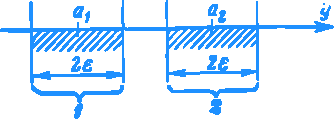
\includegraphics[width=0.55\textwidth,angle=-1]{figures/fig-09.pdf}
\caption{Proving the uniqueness of the limit.}
\label{fig-09}
\end{figure}
This proof contains at least two rather ``delicate'' points. Can you identify them?

\rdr I certainly notice one of them. If $a_{1}$ and $a_{2}$ are limits, no matter how the sequence behaves \emph{at the beginning}, its terms in the long run have to concentrate \emph{simultaneously} around $a_{1}$ and $a_{2}$ which is, of course, impossible

\athr Correct. But there is one more ``delicate'' point, namely, no matter how close $a_{1}$ and $a_{2}$ are, the; should inevitably be spaced by a segment (a gap) of a small but definitely nonzero length.

\rdr But it is self-evident.

\athr I agree. However, this ``self-evidence'' is connected to one more very fine aspect without which the very calculus could not be developed. As you probably noted, one cannot identify on the real line two neighbouring points. If one point is chosen, it is impossible, in principle, to point out its ``neighbouring'' point. In other words, no matter how carefully you select a pair of points on the real line, it is always possible to find any number of points between the two.

Take, for example, the interval $[0, 1]$. Now, exclude the point 1. You will have a half-open interval $[0, 1|$. Can you identify the largest number over this interval?

\rdr No, it is impossible.

\athr That's right. However, if there were a point neighbouring 1, after the removal of the latter this ``neighbour'' would have become the largest number. I would like to note here that many ``delicate'' points and many ``secrets'' in the calculus theorems are ultimately associated with the impossibility of identifying two neighbouring points on the real line, or of specifying the greatest or least 
number on an open interval of the real line.

But let us get back to the properties of convergent sequences and prove the following theorem:
\begin{mytheo}{Theorem}
1f sequences ($y_{n}$) and ($z_{n}$) are convergent (we denote their limits by $a$ and $b$, respectively), a sequence ($y_{n} + z_{n}$) is convergent too, its limit being $a + b$.
\end{mytheo}

\rdr This theorem is none other than rule \eqref{lim-sum} discussed in the	previous dialogue.

\athr Thats right. Nevertheless, I suggest you try to prove it.	

\rdr If we select an arbitrary $\varepsilon > 0$, then there is a number $N_{1}$ such that for all the terms of the first sequence with $n > N_{1}$ we shall have $| y_{n}- a | < \varepsilon$. In addition, for the same $\varepsilon$ there is $N_{2}$ such that for all the terms of the second sequence with $n > N_{2}$ we shall have $| z_{n}- a | < \varepsilon$. Now we select the greatest among $N_{1}$ and $N_{2}$ (we denote it by $N$), then for all $n > N$ both $| y_{n}- a | < \varepsilon$ and $| z_{n}- a | < \varepsilon$. Well, this is as far as I can go.

\athr Thus, you have established that for an arbitrary $\varepsilon$ there is $N$ such that for all $n > N$ both $| y_{n}- a | < \varepsilon$ and $| z_{n}- a | < \varepsilon$ simultaneously. And what can you say about the modulus $| (y_{n} + z_{n}) - (a +b) |$ (for all $n$)? I remind you that $|A + B | \leqslant |A| + |B|$.

\rdr Let us look at
\begin{align*}%
| (y_{n} + z_{n}) - (a +b) | & = |(y_{n}- a )+(z_{n}- b ) | \\
 & \leqslant [ |y_{n}- a| + |z_{n}- b|] \\
 & < (\varepsilon + \varepsilon ) = 2 \varepsilon 
\end{align*}

\athr You have proved the theorem, haven't you?

\rdr But we have only established that there is $N$ such that for all $n>N$ we have $|(y_{n} + z_{n})- (a+b)|< 2\varepsilon$. But we need to prove that
\begin{equation*}%
|(y_{n}+z_{n}) - (a+b) | < \varepsilon 
\end{equation*}
\athr Ah, that's peanuts, if you forgive the expression. In the case of the sequence $(y_{n} + z_{n})$ you select a value of $\varepsilon$, but for the sequences ($y_{n}$) and ($z_{n}$) you must select a e value of $\dfrac{\varepsilon}{2}$ and namely for this value find $N_{1}$ and $N_{2}$.

Thus, we have proved that if the sequences ($y_{n}$) and ($z_{n}$) are convergent, the sequence ($y_{n} + z_{n}$) is convergent too. We have even found a limit of the sum. And do you think that the converse is equally valid?

\rdr I believe it should be. 

\athr You are wrong. Here is a simple illustration:
\begin{align*}
(y_{n}) & =\frac{1}{2}, \,\frac{2}{3}, \,\frac{1}{4}, \,\frac{4}{5}, \,\frac{1}{6}, \,\frac{6}{7}, \,\frac{1}{8}, \, \ldots \\
(z_{n}) & =\frac{1}{2}, \,\frac{1}{3}, \,\frac{3}{4}, \,\frac{1}{5}, \,\frac{5}{6}, \,\frac{1}{7}, \,\frac{7}{8}, \, \ldots \\
(y_{n} + z_{n}) &= 1, \, 1,  \, 1, \, 1, \, 1, \, 1, \, 1, \ldots 
\end{align*}
As you see, the sequences $(y_{n})$ and $(z_{n})$ are not convergent, while the sequence $(y_{n}+ z_{n})$ is convergent, its limit being equal to unity.

Thus, if a sequence $(y_{n}+ z_{n})$ is convergent, two alternatives are possible:
\begin{enumerate}[label=$\textcolor{IndianRed}{\blacktriangleright}$]
\item sequences $(y_{n})$ and $(z_{n})$ are convergent as well, or 
\item sequences $(y_{n})$ and $(z_{n})$ are divergent. 
\end{enumerate}
\rdr But can it be that the sequence  $(y_{n})$ is convergent, while the sequence  $(z_{n})$ is divergent? 

\athr It may be easily shown that this is Impossible.

To begin with, let us note that if the sequence $(y_{n})$ has a limit $a$, the sequence $-(y_{n})$ is also convergent and its limit is $-a$. This follows from an easily proved equality
\begin{equation*}%
\lim\limits_{n \to \infty} (c \, y_{n}) = c \lim\limits_{n \to \infty}  y_{n}
\end{equation*}
where $c$ is a constant. Assume now that a sequence $(y_{n}+ z_{n})$ is convergent to $A$, and that $(y_{n})$ is also convergent and its limit is $a$. Let us apply the theorem on the sum of convergent sequences to the sequences $(y_{n}+ z_{n})$ and $-(y_{n})$. As a result, we obtain that the sequence  $(y_{n}+ z_{n}) - (y_{n})$, i.e. $(z_{n})$, is also convergent, with the limit $A-a$.

\rdr Indeed $(z_{n})$ cannot be divergent in this case.

\athr Very well. Let us discuss now one important particular case of convergent sequences, namely, the so-called \emph{infinitesimal sequence}, or simply, \emph{infinitesimal}. This is the name which is given to a convergent sequence with a limit equal to zero. Sequences \eqref{series-07} and \eqref{series-09} from \hyperref[infinite-seq]{Dialogue One} are examples of infinitesimals.

Note that to any convergent sequence $(y_{n})$ with a limit a there corresponds an infinitesimal sequence ($\alpha_{n}$), where $\alpha_{n} = y_{n} - a$. That is why mathematical analysis is also called calculus of infinitesimals.

Now I invite you to prove the following theorem: 
\begin{mytheo}{Theorem}
If $(y_{n})$ is a bounded sequence and ($\alpha_{n}$) is infinitesimal, then $(y_{n}\alpha_{n}$) is infinitesimal as well.
\end{mytheo}
\rdr Let us select an arbitrary  $\varepsilon > 0$. We must prove that there is $N$ such that for all $n > N$ the terms of the sequence $(y_{n}\alpha_{n}$) satisfy the inequality $|y_{n}\, \alpha_{n}| < \varepsilon$).

\athr Do you mind a hint? As the sequence $(y_{n})$ is bounded, one can find $M$ such that $| y_{n}| \leqslant M$ for any $n$.

\rdr Now all becomes very simple. We know that the sequence  ($\alpha_{n}$) is infinitesimal. It means that for any $\varepsilon' > 0$ we can find $N$ such that for all $n > N |\alpha_{n} | < \varepsilon'$. For $\varepsilon'$, I select $\dfrac{\varepsilon}{M}$ Then, for $n > N$ we have
\begin{equation*}%
|y_{n}\, \alpha_{n}| = |y_{n}| \, |\alpha_{n}|  \leqslant M |\alpha_{n}| < M \frac{\varepsilon}{M}  = \varepsilon
\end{equation*}
This completes the proof. 

\athr Excellent. Now, making use of this theorem, it is very easy to prove another theorem: 
\begin{mytheo}{Theorem}
A sequence ($y_{n}\, z_{n}$) is convergent to $ab$ if sequences ($y_{n}$) and
($z_{n}$) are convergent to $a$ and $b$, respectively.
\end{mytheo}
Suppose $y_{n} = a + \alpha_{n}$ and $z_{n} = b + \beta_{n}$. Suppose also
that the sequences ($\alpha_{n}$) and ($\beta_{n}$) are infinitesimal. Then we
can write:
\begin{equation*}%
y_{n}\, z_{n} = ab + \gamma_{n} \,\, \text{where} \,\, \gamma_{n} = b \alpha_{n} + a \beta_{n} + \alpha_{n} \beta_{n}
\end{equation*}
Making use of the theorem we have just proved, we conclude that the sequences $(b \alpha_{n}), \, (a \beta_{n}) \,\, \text{and} \,\, (\alpha_{n} \beta_{n}) $ are infinitesimal.

\rdr But what justifies your conclusion about the sequence $(\alpha_{n} \beta_{n}) $? 

\athr Because any convergent sequence (regardless of whether it is infinitesimal or not) is bounded. From the theorem on the sum of convergent sequences we infer that the sequence $(y_{n})$ is infinitesimal, which immediately yields
\begin{equation*}%
\lim\limits_{n \to \infty} (y_{n} \,z_{n}) = ab
\end{equation*}
This completes the proof. 

\rdr Perhaps we should also analyze inverse variants in which the sequence $ (y_{n} \,z_{n})$ is convergent. What can be said in this case about the sequences $(y_{n})$ and $(z_{n})$?

\athr Nothing definite. in the general case. Obviously, one possibility is that $(y_{n})$ and $(z_{n})$ are convergent. However, it is also possible, for example, for the sequence $(y_{n})$ to be convergent, while the sequence $(z_{n})$ is divergent. Here is a simple illustration:
\begin{align*}%
(y_{n}) & = 1, \, \frac{1}{4}, \, \frac{1}{9}, \, \frac{1}{16}, \, \frac{1}{25}, \, \ldots \frac{1}{n^{2}}, \, \ldots \\
(z_{n}) & =  1, \, 2, \, 3, \, 4, \, 5, \, \ldots, \, n, \, \ldots \\
(y_{n} \, z_{n}) & =   1, \, \frac{1}{2}, \, \frac{1}{3}, \, \frac{1}{4}, \, \frac{1}{5}, \, \ldots \frac{1}{n}, \, \ldots
\end{align*}
By the way, note that here we obtain an infinitesimal sequence by multiplying an infinitesimal sequence by an unbounded sequence. In the general case, however, such multiplication needn't produce an infinitesimal.

Finally, there is a possibility when the sequence $(y_{n} \, z_{n})$ is convergent, and the sequences $(y_{n})$ and $(z_{n})$ are divergent. Here is one example:
\begin{align*}%
(y_{n}) & = 1, \, \frac{1}{4}, \, 3, \, \frac{1}{16}, \, 5, \, \ldots \frac{1}{36}, \, 7, \, \ldots \\
(z_{n}) & =  1, \, 2, \, \frac{1}{9}, \, 4, \, \frac{1}{25}, \, 6, \, \frac{1}{49}, \, \ldots \\
(y_{n} \, z_{n}) & =   1, \, \frac{1}{2}, \, \frac{1}{3}, \, \frac{1}{4}, \, \frac{1}{5}, \, \frac{1}{6}, \, \frac{1}{7}, \, \ldots
\end{align*}
Now, let us formulate one more theorem: 
\begin{mytheo}{Theorem}
If $(y_{n})$ and $(z_{n})$ are sequences convergent to $a$ and $b$
when $b \neq 0$, then a sequence $\left(\dfrac{y_{n}}{z_{n}}\right)$ is also convergent, its its limit being $\dfrac{a}{b}$.
\end{mytheo}
We shall omit the proof of this theorem,

\rdr And what if the sequence $(z_{n})$ contains zero terms?

\athr Such terms are possible. Nevertheless, the number of such terms can be only finite. Do you know why? 

\rdr I think, I can guess. The sequence $(z_{n})$ has a non-zero limit $b$. 

\athr Let us specify $b > 0$.

\rdr Well, I select $\varepsilon = \dfrac{b}{2}$. There must be an integer $N$ such that $|z_{n} - b | < \dfrac{b}{2}$ for all $n > N$. Obviously all $z_{n}$ (the whole infinite ``tail'' of the sequence) will be positive. Consequently, the zero terms of the sequence $(z_{n})$ may only be encountered among a \emph{finite} number of the first $N$ terms. 

\athr Excellent. Thus, the number of zeros among the terms of $(z_{n})$ can only be finite. If such is the case, one can surely drop these terms. Indeed, \emph{an elimination of any finite number of terms of a sequence does not affect its properties}. For example, a convergent sequence still remains convergent, with its limit unaltered. An elimination of a finite number of terms may only change $N$ (for a given $\varepsilon$), which is certainly unimportant.

\rdr It is quite evident to me that by \emph{eliminating} a finite number of terms one does not affect the convergence of a sequence. But could an \emph{addition} of a finite number of terms affect the convergence of a sequence?

\athr A finite number of new terms does not affect the convergence of a sequence either. No matter how many new terms are added and what their new serial numbers are, one can always find the greatest number $N$ after which the whole infinite ``tail'' of the sequence is unchanged. No matter how large the number of new terms may be and where you insert them, the finite set of new terms cannot change the infinite ``tail'' of the sequence. And it is the ``tail'' that determines the convergence (divergence) of a sequence.

Thus, we have arrived at the following: 
\begin{mytheo}{Conclusion}
Elimination, addition, and any other change of a finite number of terms of a sequence do not affect either its convergence or its limit (if the sequence is convergent).
\end{mytheo}

\rdr I guess that an elimination of an infinite number of terms (for example, every other term) must not affect the convergence of a sequence either.

\athr Here you must be very careful. If an initial sequence is convergent, an elimination of an infinite number of its terms (provided that the number of the remaining terms is also infinite) does not affect either convergence or the limit of the sequence. If, however, an initial sequence is divergent, an elimination of an infinite number of its terms may, in certain cases, convert the sequence into a convergent one. For example, if you eliminate from divergent sequence \eqref{series-10} (see \hyperref[infinite-seq]{Dialogue One}) all the terms with even serial numbers, you will get the convergent sequence.
\begin{equation*}%
1, \, \frac{1}{3}, \, \frac{1}{5}, \,\frac{1}{7}, \,\frac{1}{9}, \,\frac{1}{11}, \,\frac{1}{13}, \, \ldots
\end{equation*}
Suppose we form from a given convergent sequence two new convergent sequences. The first new sequence will consist of the terms of the initial sequence with \emph{odd} serial numbers, while the second will consists of the terms with \emph{even} serial numbers. What do you think are the limits of these new sequences?

\rdr It is easy to prove that the new sequences will have the same limit as the initial sequence.

\athr You are right. 

Note that from a given convergent sequence we can form not only two but a \emph{finite number} $m$ of new sequences converging to the same limit. One way to do it is as follows. The first	new sequence will consist of the 1st, $(m + 1)$st, $(2m + 1)$st, $(3m + 1)$st, etc., terms of the initial sequence. The second	sequence will consist of the 2nd, $(m + 2)$nd, $(2m + 2)$nd, $(3m + 2)$nd, etc., terms of the initial sequence.

Similarly we can form the third, the fourth, and other sequences.

In conclusion, let us see how one can ``spoil'' a convergent sequence by turning it into divergent. Clearly, different ``spoiling'' approaches are possible. Try to suggest something simple.

\rdr For example, we can replace all the terms with even serial numbers by a constant that is not equal to the limit of the initial sequence. For example, convergent sequence \eqref{series-05} (see \hyperref[infinite-seq]{Dialogue One})  can be ``spoilt'' in the following manner:
\begin{equation*}%
\frac{1}{2}, \, 2, \, \frac{3}{4}, \, 2, \, \frac{5}{6}, \, 2, \, \frac{7}{8}, \, 2,  \, \ldots
\end{equation*}

\athr I see that you have mastered very well the essence of the concept of a convergent sequence. Now we are ready for another substantial step, namely, consider one of the most important concepts in calculus: the definition of a function.
}